\section{\gls{bc} level matching distribution}
In this section, the distribution for the \gls{bc} level versus \gls{ac} level will be analysed. The analysis is done to verify the distribution of both the initial test, the familiarization test and the matching test part of the \gls{bier} test. Because of the limited number of test subjects, there will be done a fourth analysis where all matching data is merged to one data called Total data. This include also the familiarization and \gls{bier} result although the data is from the same test subjects. The reasons to bring both familiarization and \gls{bier} intro the Total data is because they mostly had small difference matching opinion in the \gls{bier} compare to the familiarization.


This analysis will estimate the data distribution based on the subject data. It is assumed that the the distribution is a Gaussian distribution and therefore the data will be compared to the \gls{pdf} and the \gls{cdf} of a Gaussian distribution. The comparing will be done by calculating the \gls{mse} between the subject result and the \gls{pdf} and as a visualize look at the \gls{cdf} plot. The \gls{mse} will be calculated with the MATLAB function \texttt{immse}. In the end the 25 \textsuperscript{th} and 75\textsuperscript{th} percentile will be present. If the Gaussian hypnotises can be concluded to be correct, it can then be assumed that a greater field test will approximate result in the same distribution.

To calculate the \gls{pdf} and \gls{cdf} based on the subject data, the input for the function have to be defined based on the subject data. The input samples for calculating the  \gls{pdf} will be the average matching level for every subjects average matching level, and the variance will be calculated based on the average matching level for every subject. The following \autoref{sec:pdf_of_bc} shows the calculated average and variance. 

\begin{table}[H]
\centering
\caption{The average and variance.}
\begin{tabular}{l|ll}
Matching test                 & $\mu$ & $\sigma^2$ \\ \hline
Initial                       & 50    & 5.34       \\
Familiarization of \gls{bier} & 49.48 & 4.604      \\
\gls{bier}                    & 47.99 & 9.44      \\
Total                    & 49.10 & 6.82      
\end{tabular}
\label{sec:pdf_of_bc}
\end{table}

 The Gaussian \gls{pdf} is calculated as following \autoref{eq:pdf_of_bc} where the \gls{cdf} plot is calculated by using the MATLAB function \texttt{normplot}

\begin{equation}\label{eq:pdf_of_bc}
f(x_{k}) = \frac{1}{\sqrt{2 \pi \sigma^2}}e^{-\frac{(x-\mu)^2}{2\sigma^2}}
\end{equation}


The following six figurers display the data from the subject as a histogram to compare with the \gls{pdf} function and as dots to compare with \gls{cdf} function. The Gaussian \gls{pdf} and \gls{cdf} is calculated according to \autoref{eq:pdf_of_bc} with the use of the data in \autoref{sec:pdf_of_bc}.


The following \autoref{fig:initial_pdf} and \autoref{fig:initial_normplot} shows the data for the initial test.

 \begin{figure}[H]
	\centering
	% This file was created by matlab2tikz.
%
%The latest updates can be retrieved from
%  http://www.mathworks.com/matlabcentral/fileexchange/22022-matlab2tikz-matlab2tikz
%where you can also make suggestions and rate matlab2tikz.
%
\definecolor{mycolor1}{rgb}{0.00000,0.44700,0.74100}%
\definecolor{mycolor2}{rgb}{0.85000,0.32500,0.09800}%
%
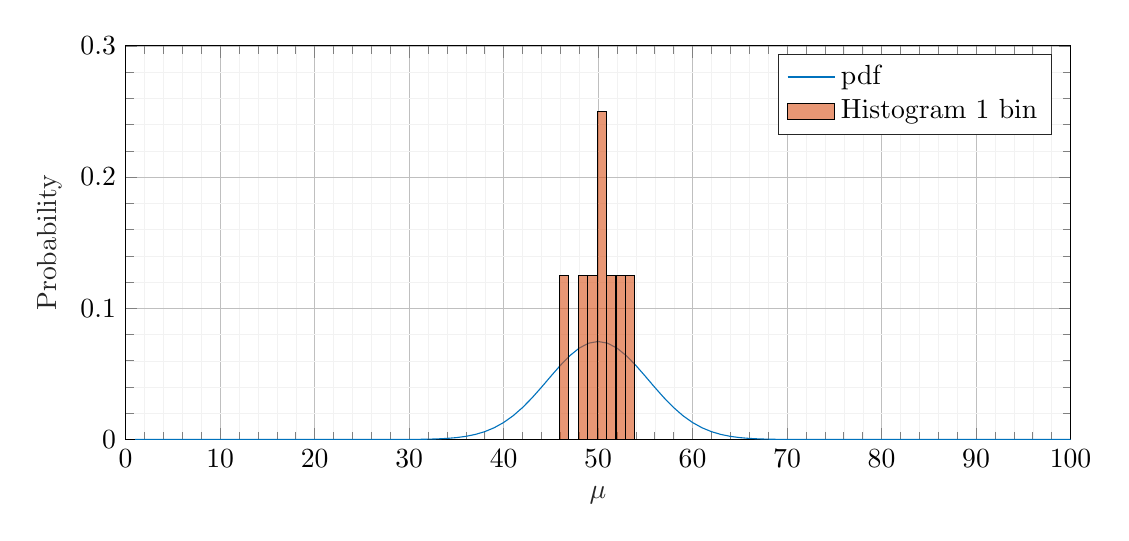
\begin{tikzpicture}

\begin{axis}[%
width=120mm, 
height=50mm, 
at={(5mm,5mm)}, 
scale only axis,
xmin=0,
xmax=100,
xlabel style={font=\color{white!15!black}},
xlabel={$\mu$ \si{\decibel}},
ylabel style={font=\color{white!15!black}},
ylabel={Probability},
ymin=0,
ymax=0.3,
axis background/.style={fill=white},
grid=both,
grid style={line width=.1pt, draw=gray!10},
major grid style={line width=.2pt,draw=gray!50}, 
minor tick num=4,
legend style={legend cell align=left, align=left, draw=white!15!black}
]
\addplot [color=mycolor1]
  table[row sep=crcr]{%
1	3.88753288613558e-20\\
2	2.12976799844824e-19\\
3	1.12657588814019e-18\\
4	5.75385005814751e-18\\
5	2.83743918600713e-17\\
6	1.3510285222346e-16\\
7	6.21115556627748e-16\\
8	2.75708547023195e-15\\
9	1.18167483212333e-14\\
10	4.89007675257209e-14\\
11	1.95390434710717e-13\\
12	7.53808197778718e-13\\
13	2.80794338283003e-12\\
14	1.00991720510473e-11\\
15	3.50714021086796e-11\\
16	1.1759542340013e-10\\
17	3.80712945984117e-10\\
18	1.19007629221712e-09\\
19	3.59188063425429e-09\\
20	1.04674024307622e-08\\
21	2.94527520111863e-08\\
22	8.0017093744719e-08\\
23	2.09898628090369e-07\\
24	5.3162618044904e-07\\
25	1.3000889099313e-06\\
26	3.06979716636403e-06\\
27	6.99868169040538e-06\\
28	1.54061008341285e-05\\
29	3.2744560372424e-05\\
30	6.7197872825729e-05\\
31	0.000133150199239833\\
32	0.000254740530757393\\
33	0.000470569973179873\\
34	0.00083930596077183\\
35	0.00144539429743596\\
36	0.00240337920955625\\
37	0.00385858610996265\\
38	0.00598141625771222\\
39	0.00895261257146183\\
40	0.0129379505820961\\
41	0.0180530721954509\\
42	0.024322414391658\\
43	0.0316396872231062\\
44	0.0397399771717304\\
45	0.0481940005845401\\
46	0.0564323683975447\\
47	0.0638018849939972\\
48	0.0696480041930907\\
49	0.0734097551585918\\
50	0.0747082922100061\\
51	0.0734097551585918\\
52	0.0696480041930907\\
53	0.0638018849939972\\
54	0.0564323683975447\\
55	0.0481940005845401\\
56	0.0397399771717304\\
57	0.0316396872231062\\
58	0.024322414391658\\
59	0.0180530721954509\\
60	0.0129379505820961\\
61	0.00895261257146183\\
62	0.00598141625771222\\
63	0.00385858610996265\\
64	0.00240337920955625\\
65	0.00144539429743596\\
66	0.00083930596077183\\
67	0.000470569973179873\\
68	0.000254740530757393\\
69	0.000133150199239833\\
70	6.7197872825729e-05\\
71	3.2744560372424e-05\\
72	1.54061008341285e-05\\
73	6.99868169040538e-06\\
74	3.06979716636403e-06\\
75	1.3000889099313e-06\\
76	5.3162618044904e-07\\
77	2.09898628090369e-07\\
78	8.0017093744719e-08\\
79	2.94527520111863e-08\\
80	1.04674024307622e-08\\
81	3.59188063425429e-09\\
82	1.19007629221712e-09\\
83	3.80712945984117e-10\\
84	1.1759542340013e-10\\
85	3.50714021086796e-11\\
86	1.00991720510473e-11\\
87	2.80794338283003e-12\\
88	7.53808197778718e-13\\
89	1.95390434710717e-13\\
90	4.89007675257209e-14\\
91	1.18167483212333e-14\\
92	2.75708547023195e-15\\
93	6.21115556627748e-16\\
94	1.3510285222346e-16\\
95	2.83743918600713e-17\\
96	5.75385005814751e-18\\
97	1.12657588814019e-18\\
98	2.12976799844824e-19\\
99	3.88753288613558e-20\\
100	6.85150199158635e-21\\
};

\addplot[ybar interval, fill=mycolor2, fill opacity=0.6, draw=black, area legend] table[row sep=crcr] {%
x	y\\
45.9	0.125\\
46.9	0\\
47.9	0.125\\
48.9	0.125\\
49.9	0.25\\
50.9	0.125\\
51.9	0.125\\
52.9	0.125\\
53.9	0.125\\
};

\addlegendentry{\gls{pdf}}
\addlegendentry{Histogram \SI{1}{\decibel} bin}

\end{axis}
\end{tikzpicture}%
		\caption{The plot shows the Gaussian \gls{pdf} as the blue line with the initial data in \autoref{sec:pdf_of_bc}. The histogram is based on the mean data in \autoref{apend:match_field_init}}
		\label{fig:initial_pdf}
\end{figure}

\plot{chapters/tests/initial_normplot}{The plot shows the Gaussian \gls{cdf} as the blue line with the initial data in \autoref{sec:pdf_of_bc}. The histogram is based on the mean data in \autoref{apend:match_field_init}}{fig:initial_normplot}

It can be seen in \autoref{fig:initial_pdf} and \autoref{fig:initial_normplot} that the measured data, might be a Gaussian distribution. There is no outliers of the \gls{pdf} and the highest probability lays close to the highest probability of the Gaussian \gls{pdf}. It can also be seen that the subject data compare to the \gls{cdf} mostly follows the line. The calculated \gls{mse} between the data and the Gaussian \gls{pdf} is $11.835 \cdot 10^{-5}$

The following \autoref{fig:fam_pdf} and autoref{fig:fam_normplot}  shows the data for the familiarization test.

 \begin{figure}[H]
	\centering
	% This file was created by matlab2tikz.
%
%The latest updates can be retrieved from
%  http://www.mathworks.com/matlabcentral/fileexchange/22022-matlab2tikz-matlab2tikz
%where you can also make suggestions and rate matlab2tikz.
%
%
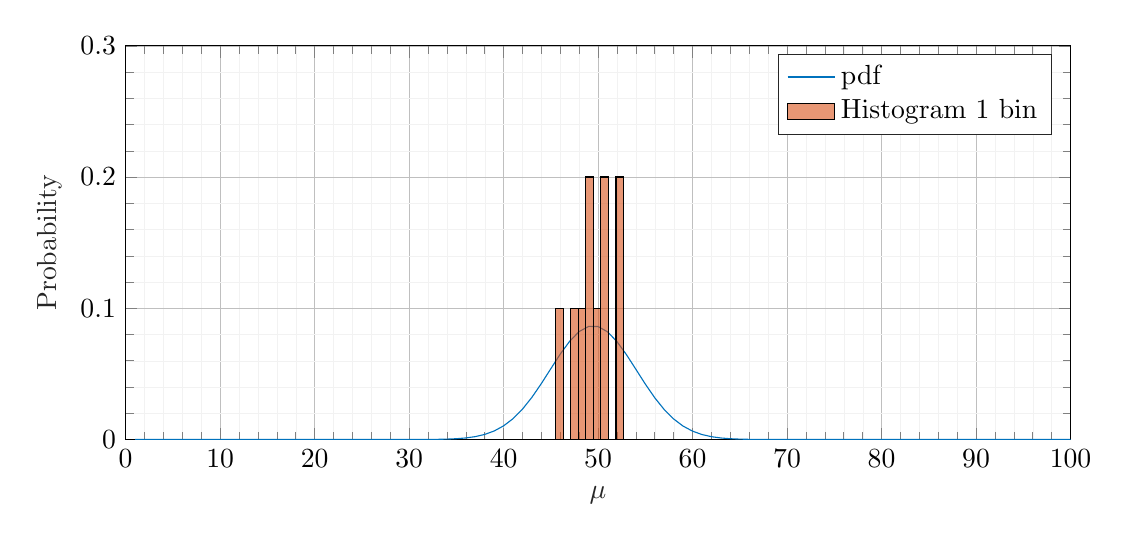
\begin{tikzpicture}

\begin{axis}[%
width=120mm, 
height=50mm, 
at={(5mm,5mm)}, 
scale only axis,
xmin=0,
xmax=100,
xlabel style={font=\color{white!15!black}},
xlabel={$\mu$ \si{\decibel}},
ymin=0,
ymax=0.3,
ylabel style={font=\color{white!15!black}},
ylabel={Probability},
axis background/.style={fill=white},
grid=both,
grid style={line width=.1pt, draw=gray!10},
major grid style={line width=.2pt,draw=gray!50}, 
minor tick num=4,
legend style={legend cell align=left, align=left, draw=white!15!black}
]
\addplot [color=mycolor1]
  table[row sep=crcr]{%
1	7.25124262285027e-26\\
2	6.9736256148195e-25\\
3	6.3975863118078e-24\\
4	5.59867185198651e-23\\
5	4.67374708419392e-22\\
6	3.72183173806484e-21\\
7	2.8272199511126e-20\\
8	2.04867842033147e-19\\
9	1.41611760802938e-18\\
10	9.3376198028466e-18\\
11	5.87332975885434e-17\\
12	3.52406505713514e-16\\
13	2.01704126654263e-15\\
14	1.10127805158289e-14\\
15	5.73575402083945e-14\\
16	2.8496753564529e-13\\
17	1.35055286711742e-12\\
18	6.10575151391139e-12\\
19	2.63316453103856e-11\\
20	1.08324876156756e-10\\
21	4.25098663916887e-10\\
22	1.59133865697685e-09\\
23	5.68259650324332e-09\\
24	1.93571921328358e-08\\
25	6.28997958358421e-08\\
26	1.94969844315782e-07\\
27	5.76496915633775e-07\\
28	1.6260648626584e-06\\
29	4.37512108158142e-06\\
30	1.12293242400631e-05\\
31	2.74934032163068e-05\\
32	6.42117808716936e-05\\
33	0.00014305803734214\\
34	0.000304033293539703\\
35	0.000616369811686115\\
36	0.0011919908169594\\
37	0.00219895222295159\\
38	0.00386963507900279\\
39	0.00649584365155497\\
40	0.0104018946119547\\
41	0.015889150163673\\
42	0.0231526242531135\\
43	0.0321818578233708\\
44	0.042671050443305\\
45	0.0539717985238587\\
46	0.0651196084986405\\
47	0.074949373230504\\
48	0.0822878213165313\\
49	0.0861815809197056\\
50	0.0861003036789081\\
51	0.082055225623091\\
52	0.074596618095108\\
53	0.0646909259841801\\
54	0.053515419063359\\
55	0.0422304615133424\\
56	0.0317895264614316\\
57	0.0228272515066231\\
58	0.0156363190375106\\
59	0.0102170791146777\\
60	0.00636839985272433\\
61	0.00378656333233425\\
62	0.00214768933487952\\
63	0.00116200776455885\\
64	0.000599732982459356\\
65	0.000295269216252836\\
66	0.00013867230774276\\
67	6.21258936366136e-05\\
68	2.6550144473938e-05\\
69	1.08236181584675e-05\\
70	4.20910122803692e-06\\
71	1.56141235907502e-06\\
72	5.52531686266294e-07\\
73	1.865125668e-07\\
74	6.00579277538243e-08\\
75	1.84477719592347e-08\\
76	5.40541240361262e-09\\
77	1.51086298105428e-09\\
78	4.02840068197562e-10\\
79	1.02459345045515e-10\\
80	2.48588952332569e-11\\
81	5.75338460259697e-12\\
82	1.27021232816772e-12\\
83	2.67510340619409e-13\\
84	5.37422889032833e-14\\
85	1.02991901922856e-14\\
86	1.88278760805374e-15\\
87	3.28330265865536e-16\\
88	5.4617502786363e-17\\
89	8.66690616845009e-18\\
90	1.31192100039415e-18\\
91	1.89436040352638e-19\\
92	2.60932914288211e-20\\
93	3.42851817693177e-21\\
94	4.29729711525362e-22\\
95	5.138018237565e-23\\
96	5.86012979396047e-24\\
97	6.37573360669493e-25\\
98	6.61705012857993e-26\\
99	6.55103652169519e-27\\
100	6.18681244638774e-28\\
};

\addplot[ybar interval, fill=mycolor2, fill opacity=0.6, draw=black, area legend] table[row sep=crcr] {%
x	y\\
45.5	0.1\\
46.3	0\\
47.1	0.1\\
47.9	0.1\\
48.7	0.2\\
49.5	0.1\\
50.3	0.2\\
51.1	0\\
51.9	0.2\\
52.7	0.2\\
};

\addlegendentry{\gls{pdf}}
\addlegendentry{Histogram \SI{1}{\decibel} bin}

\end{axis}
\end{tikzpicture}%
		\caption{The plot shows the Gaussian  \gls{pdf} as the blue line with the initial data in \autoref{sec:pdf_of_bc}. The histogram is based on the mean data in \autoref{apend:matching_in_bier}}
		\label{fig:fam_pdf}
\end{figure}

 \begin{figure}[H]
	\centering
	% This file was created by matlab2tikz.

%The latest updates can be retrieved from
%  http://www.mathworks.com/matlabcentral/fileexchange/22022-matlab2tikz-matlab2tikz
%where you can also make suggestions and rate matlab2tikz.
%
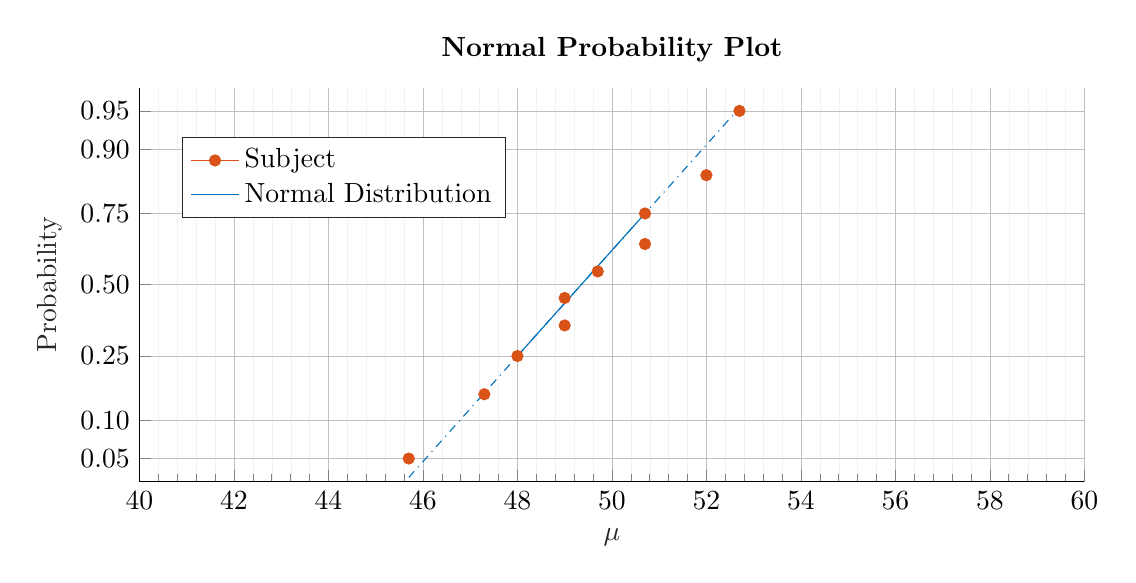
\begin{tikzpicture}

\begin{axis}[%
width=120mm, 
height=50mm, 
at={(5mm,5mm)}, 
scale only axis,
xmin=40,
xmax=60,
xlabel style={font=\color{white!15!black}},
xlabel={$\mu$ \si{\decibel}},
ymin=-1.86273186742165,
ymax=1.86273186742165,
ytick={-3.09023230616781,-2.74778138544499,-2.32634787404084,-2.05374891063182,-1.64485362695147,-1.2815515655446,-0.674489750196082,0,0.674489750196082,1.2815515655446,1.64485362695147,2.05374891063182,2.32634787404084,2.74778138544499,3.09023230616781},
yticklabels={{0.001},{0.003},{0.01},{0.02},{0.05},{0.10},{0.25},{0.50},{0.75},{0.90},{0.95},{0.98},{0.99},{0.997},{0.999}},
ylabel style={font=\color{white!15!black}},
ylabel={Probability},
axis background/.style={fill=white},
title style={font=\bfseries},
title={Normal Probability Plot},
axis x line*=bottom,
axis y line*=left,
grid=both,
grid style={line width=.1pt, draw=gray!10},
major grid style={line width=.2pt,draw=gray!50}, 
minor tick num=4,
legend style={at={(0.045,0.669)}, anchor=south west, legend cell align=left, align=left, draw=white!15!black}
]

\addplot [color=mycolor2, draw=none, mark=*, mark options={solid, mycolor2}]
  table[row sep=crcr]{%
45.7	-1.64485362695147\\
47.3	-1.03643338949379\\
48	-0.674489750196082\\
49	-0.385320466407568\\
49	-0.125661346855074\\
49.7	0.125661346855074\\
50.7	0.385320466407568\\
50.7	0.674489750196082\\
52	1.03643338949379\\
52.7	1.64485362695147\\
};
\addlegendentry{Subject}

\addplot [color=mycolor1]
  table[row sep=crcr]{%
48	-0.674489750196082\\
50.7	0.674489750196082\\
};
\addlegendentry{Normal Distribution}

\addplot [color=mycolor1, dashdotted]
  table[row sep=crcr]{%
45.7	-1.82362043571533\\
52.7	1.67373382456065\\
};
%\addlegendentry{data1}





\end{axis}
\end{tikzpicture}%
		\caption{The plot shows the Gaussian  \gls{pdf} as the blue line with the initial data in \autoref{sec:pdf_of_bc}. The histogram is based on the mean data in \autoref{apend:matching_in_bier}}
		\label{fig:fam_normplot}
\end{figure}

It can be seen in \autoref{fig:fam_pdf} and autoref{fig:fam_normplot}  that the measured data might be a Gaussian distribution. There is no outliers of the \gls{pdf} and two the highest probability lays close to the highest probability of the Gaussian \gls{pdf}, but there is also one histogram bar that have high probability but lays at the high end of the test subject mean. It can also be seen that the subject data compare to the \gls{cdf} mostly follows the line. The calculated \gls{mse} between the data and the Gaussian distribution function is $13.311 \cdot 10^{-5}$

The following \autoref{fig:bier_pdf} and \autoref{fig:bier_normplot} shows the data for the \gls{bier} test.
 \begin{figure}[H]
	\centering
	% This file was created by matlab2tikz.
%
%The latest updates can be retrieved from
%  http://www.mathworks.com/matlabcentral/fileexchange/22022-matlab2tikz-matlab2tikz
%where you can also make suggestions and rate matlab2tikz.
%
%
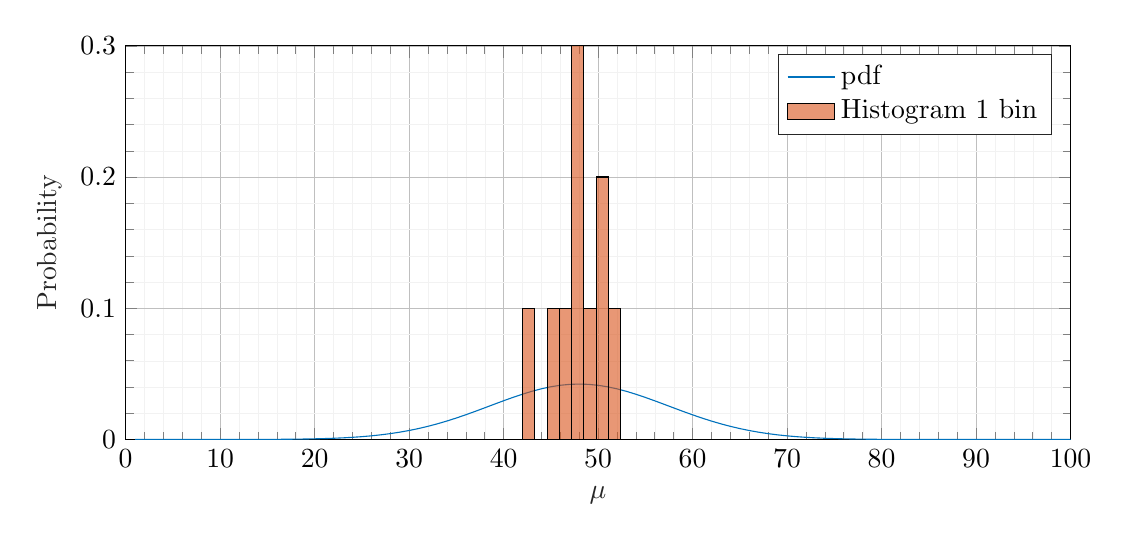
\begin{tikzpicture}

\begin{axis}[%
width=120mm, 
height=50mm, 
at={(5mm,5mm)}, 
scale only axis,
xmin=0,
xmax=100,
xlabel style={font=\color{white!15!black}},
xlabel={$\mu$ \si{\decibel}},
ymin=0,
ymax=0.3,
ylabel style={font=\color{white!15!black}},
ylabel={Probability},
axis background/.style={fill=white},
grid=both,
grid style={line width=.1pt, draw=gray!10},
major grid style={line width=.2pt,draw=gray!50}, 
minor tick num=4,
legend style={legend cell align=left, align=left, draw=white!15!black}
]
\addplot [color=mycolor1]
  table[row sep=crcr]{%
1	1.75976893619116e-07\\
2	2.96499745056968e-07\\
3	4.93991536925927e-07\\
4	8.13844064187308e-07\\
5	1.32583475470207e-06\\
6	2.13581732660697e-06\\
7	3.40224291852152e-06\\
8	5.35911454274503e-06\\
9	8.34732393453135e-06\\
10	1.28566553755954e-05\\
11	1.95810170354727e-05\\
12	2.94896076905044e-05\\
13	4.39166548273957e-05\\
14	6.46719589849264e-05\\
15	9.41736250152641e-05\\
16	0.000135602927916385\\
17	0.000193079138766793\\
18	0.000271849254501927\\
19	0.000378483932135175\\
20	0.000521066622631758\\
21	0.000709358161969407\\
22	0.000954914290311572\\
23	0.00127112927911342\\
24	0.00167317574151511\\
25	0.00217780957859338\\
26	0.0028030106971015\\
27	0.00356743537056704\\
28	0.00448966544515434\\
29	0.00558725320592597\\
30	0.00687557832773972\\
31	0.00836655406580708\\
32	0.010067242198247\\
33	0.0119784581374744\\
34	0.0140934665522146\\
35	0.0163968810479707\\
36	0.0188638863082879\\
37	0.0214598954485423\\
38	0.0241407378815024\\
39	0.0268534436253593\\
40	0.0295376499824088\\
41	0.032127608608523\\
42	0.0345547192081637\\
43	0.0367504654059601\\
44	0.0386495841689526\\
45	0.04019326767272\\
46	0.0413321800173968\\
47	0.0420290735000968\\
48	0.0422608110765178\\
49	0.0420196418628372\\
50	0.0413136316004929\\
51	0.0401662147382492\\
52	0.0386149028265732\\
53	0.0367092485175083\\
54	0.0345082192835356\\
55	0.0320771748484953\\
56	0.0294846638631276\\
57	0.0267992572672885\\
58	0.0240866189405342\\
59	0.0214069814817918\\
60	0.0188131505990801\\
61	0.0163491108319253\\
62	0.0140492535748875\\
63	0.0119382005850894\\
64	0.0100311563447815\\
65	0.00833469351204139\\
66	0.00684785848176511\\
67	0.00556347865475572\\
68	0.00446955805759455\\
69	0.00355066130314675\\
70	0.00278920489270886\\
71	0.00216659679796413\\
72	0.00166418760427849\\
73	0.00126401717780078\\
74	0.000949358354038619\\
75	0.000705072675158925\\
76	0.000517802447663675\\
77	0.000376028551051798\\
78	0.000270025047238332\\
79	0.00019174046994973\\
80	0.000134632537568948\\
81	9.34787255540803e-05\\
82	6.41803441194286e-05\\
83	4.35730346184298e-05\\
84	2.9252304145117e-05\\
85	1.94190893784903e-05\\
86	1.27474743937922e-05\\
87	8.27457969539329e-06\\
88	5.31121944111089e-06\\
89	3.37107996709413e-06\\
90	2.11577933715202e-06\\
91	1.31310119158659e-06\\
92	8.05846876076769e-07\\
93	4.89027593725223e-07\\
94	2.93454457660743e-07\\
95	1.74130386509985e-07\\
96	1.02172712748421e-07\\
97	5.92818559724943e-08\\
98	3.40122346612011e-08\\
99	1.92963447144267e-08\\
100	1.08253373275121e-08\\
};

\addplot[ybar interval, fill=mycolor2, fill opacity=0.6, draw=black, area legend] table[row sep=crcr] {%
x	y\\
42	0.1\\
43.3	0\\
44.6	0.1\\
45.9	0.1\\
47.2	0.3\\
48.5	0.1\\
49.8	0.2\\
51.1	0.1\\
52.4	0.1\\
};

\addlegendentry{\gls{pdf}}
\addlegendentry{Histogram \SI{1}{\decibel} bin}

\end{axis}
\end{tikzpicture}%
		\caption{The plot shows the Gaussian  \gls{pdf} as the blue line with the initial data in \autoref{sec:pdf_of_bc}. The histogram is based on the mean data in \autoref{apend:matching_in_bier}}
		\label{fig:bier_pdf}
\end{figure}

 \begin{figure}[H]
	\centering
	% This file was created by matlab2tikz.


%The latest updates can be retrieved from
%  http://www.mathworks.com/matlabcentral/fileexchange/22022-matlab2tikz-matlab2tikz
%where you can also make suggestions and rate matlab2tikz.
%
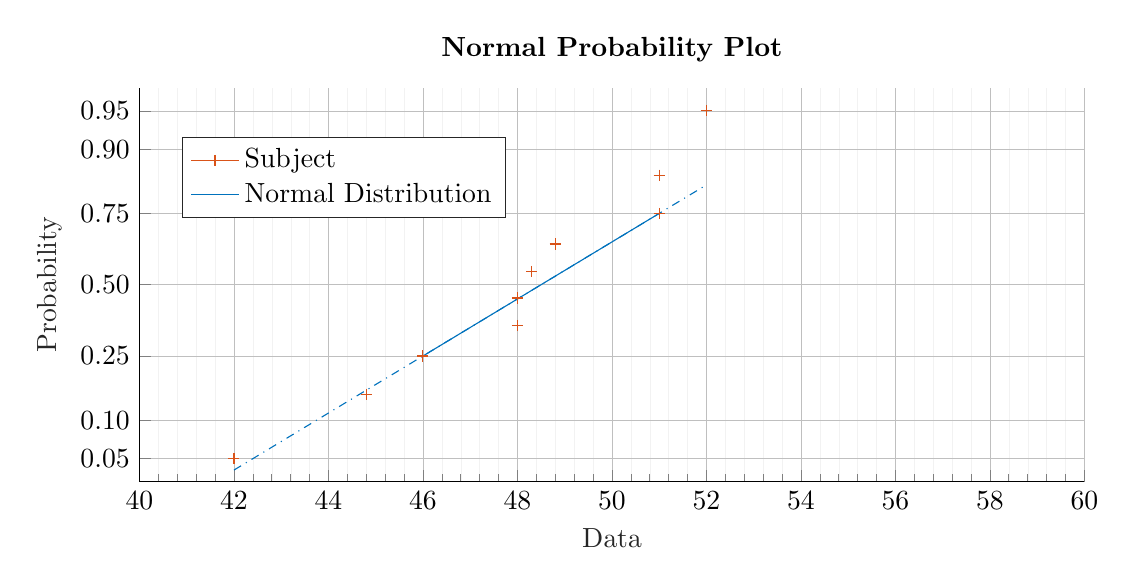
\begin{tikzpicture}

\begin{axis}[%
width=120mm, 
height=50mm, 
at={(5mm,5mm)}, 
scale only axis,
xmin=40,
xmax=60,
xlabel style={font=\color{white!15!black}},
xlabel={Data},
ymin=-1.86273186742165,
ymax=1.86273186742165,
ytick={-3.09023230616781,-2.74778138544499,-2.32634787404084,-2.05374891063182,-1.64485362695147,-1.2815515655446,-0.674489750196082,0,0.674489750196082,1.2815515655446,1.64485362695147,2.05374891063182,2.32634787404084,2.74778138544499,3.09023230616781},
yticklabels={{0.001},{0.003},{0.01},{0.02},{0.05},{0.10},{0.25},{0.50},{0.75},{0.90},{0.95},{0.98},{0.99},{0.997},{0.999}},
ylabel style={font=\color{white!15!black}},
ylabel={Probability},
axis background/.style={fill=white},
title style={font=\bfseries},
title={Normal Probability Plot},
axis x line*=bottom,
axis y line*=left,
grid=both,
grid style={line width=.1pt, draw=gray!10},
major grid style={line width=.2pt,draw=gray!50}, 
minor tick num=4,
legend style={at={(0.045,0.669)}, anchor=south west, legend cell align=left, align=left, draw=white!15!black}
]

\addplot [color=mycolor2, draw=none, mark=+, mark options={solid, mycolor2}]
  table[row sep=crcr]{%
42	-1.64485362695147\\
44.8	-1.03643338949379\\
46	-0.674489750196082\\
48	-0.385320466407568\\
48	-0.125661346855074\\
48.3	0.125661346855074\\
48.8	0.385320466407568\\
51	0.674489750196082\\
51	1.03643338949379\\
52	1.64485362695147\\
};
\addlegendentry{Subject}

\addplot [color=mycolor1]
  table[row sep=crcr]{%
46	-0.674489750196082\\
51	0.674489750196082\\
};
\addlegendentry{Normal Distribution}

\addplot [color=mycolor1, dashdotted]
  table[row sep=crcr]{%
42	-1.75367335050981\\
52	0.944285650274515\\
};
%\addlegendentry{data1}





\end{axis}
\end{tikzpicture}%
		\caption{The plot shows the Gaussian  \gls{pdf} as the blue line with the initial data in \autoref{sec:pdf_of_bc}. The histogram is based on the mean data in \autoref{apend:matching_in_bier}}
		\label{fig:bier_normplot}
\end{figure}

It can be seen in \autoref{fig:bier_pdf} and \autoref{fig:bier_normplot} that the measured data for the \gls{bier} test have the same tendency as in initial test \autoref{fig:fam_pdf} and the familiarization test \autoref{fig:initial_pdf}. The distribution might be a Gaussian distribution. There is no outliers and the highest probability lays close to the highest probability of the Gaussian distribution.  It can also be seen that the subject data compare to the \gls{cdf} mostly follows the line. The calculated \gls{mse} between the data and the Gaussian distribution function is $13.339 \cdot 10^{-5}$.



To include more data in the comparison between test subject and the Gaussian \gls{pdf}, all present subject data is merged to one data file, where the mean and variance is calculated. The following figure \autoref{fig:total_pdf} and \autoref{fig:total_normplot} shows the merged subject data compared with the Gaussian \gls{pdf}.


 \begin{figure}[H]
	\centering
	% This file was created by matlab2tikz.
%
%The latest updates can be retrieved from
%  http://www.mathworks.com/matlabcentral/fileexchange/22022-matlab2tikz-matlab2tikz
%where you can also make suggestions and rate matlab2tikz.
%
\definecolor{mycolor1}{rgb}{0.00000,0.44700,0.74100}%
\definecolor{mycolor2}{rgb}{0.85000,0.32500,0.09800}%
%
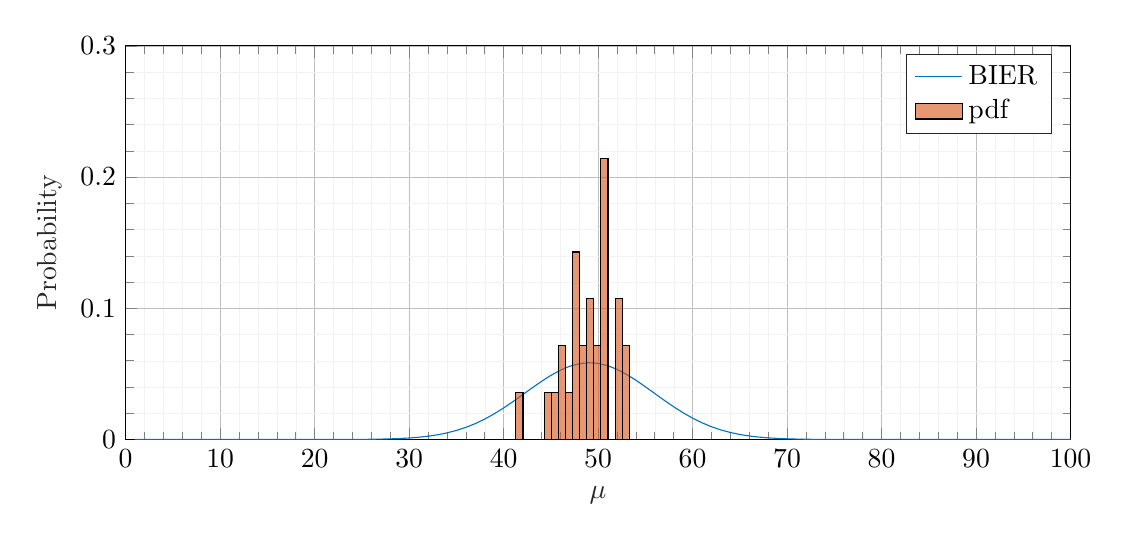
\begin{tikzpicture}

\begin{axis}[%
width=120mm, 
height=50mm, 
at={(5mm,5mm)}, 
scale only axis,
xmin=0,
xmax=100,
xlabel style={font=\color{white!15!black}},
xlabel={$\mu$ \si{\decibel}},
ymin=0,
ymax=0.30,
ylabel style={font=\color{white!15!black}},
ylabel={Probability},
axis background/.style={fill=white},
grid=both,
grid style={line width=.1pt, draw=gray!10},
major grid style={line width=.2pt,draw=gray!50}, 
minor tick num=4,
legend style={legend cell align=left, align=left, draw=white!15!black}
]
\addplot [color=mycolor1]
  table[row sep=crcr]{%
1	9.01034219754882e-13\\
2	2.51009812523995e-12\\
3	6.84371216299437e-12\\
4	1.82618341101851e-11\\
5	4.76923445786109e-11\\
6	1.21900243922119e-10\\
7	3.04938386502976e-10\\
8	7.46571218574015e-10\\
9	1.78888330197399e-09\\
10	4.19512010515232e-09\\
11	9.62849501156914e-09\\
12	2.16283825351717e-08\\
13	4.75489900114573e-08\\
14	1.02308136121882e-07\\
15	2.15442148078078e-07\\
16	4.44020263631701e-07\\
17	8.95625668557875e-07\\
18	1.76807993391386e-06\\
19	3.41608666887847e-06\\
20	6.45962769117923e-06\\
21	1.19546734198352e-05\\
22	2.16530743513101e-05\\
23	3.83842482705996e-05\\
24	6.65944649561856e-05\\
25	0.000113077148999278\\
26	0.000187915752794269\\
27	0.000305635043364694\\
28	0.000486513313743516\\
29	0.000757945419875085\\
30	0.00115566712237925\\
31	0.00172456356014809\\
32	0.00251870482513029\\
33	0.00360020279614776\\
34	0.00503649349545217\\
35	0.00689574529471229\\
36	0.00924029354194626\\
37	0.0121183068715824\\
38	0.0155542740229358\\
39	0.0195393074874385\\
40	0.0240226111137723\\
41	0.0289056590741951\\
42	0.0340405966182711\\
43	0.0392340437594224\\
44	0.0442568605243411\\
45	0.048859582925442\\
46	0.0527922934980413\\
47	0.0558268245874159\\
48	0.0577785906263479\\
49	0.0585251565242688\\
50	0.0580189474172002\\
51	0.0562922657201139\\
52	0.0534538799965585\\
53	0.0496776863857804\\
54	0.0451850857088073\\
55	0.0402235577610565\\
56	0.0350443067991965\\
57	0.0298817541406269\\
58	0.0249371216785499\\
59	0.0203675214538613\\
60	0.0162810219686386\\
61	0.0127372819976759\\
62	0.00975266906177582\\
63	0.00730839198816506\\
64	0.00536008652082168\\
65	0.00384745358218745\\
66	0.00270287897336577\\
67	0.00185836677537929\\
68	0.0012505120668009\\
69	0.000823561361788729\\
70	0.000530830246877145\\
71	0.00033486285914331\\
72	0.000206742575759036\\
73	0.00012492359862392\\
74	7.38772416156205e-05\\
75	4.27590924467894e-05\\
76	2.4221325601087e-05\\
77	1.34282357931694e-05\\
78	7.28604134400339e-06\\
79	3.86915319722988e-06\\
80	2.01090633378741e-06\\
81	1.02286750074447e-06\\
82	5.09211894985224e-07\\
83	2.48101461039605e-07\\
84	1.18307349664425e-07\\
85	5.5213560092053e-08\\
86	2.52192053490206e-08\\
87	1.12737569318095e-08\\
88	4.93239169477602e-09\\
89	2.11202021396818e-09\\
90	8.85095647245183e-10\\
91	3.6302284939487e-10\\
92	1.45723414699552e-10\\
93	5.72501118305298e-11\\
94	2.20127834432921e-11\\
95	8.28371606945251e-12\\
96	3.05089365792487e-12\\
97	1.09971603446035e-12\\
98	3.87958852761604e-13\\
99	1.33949901095746e-13\\
100	4.52637727767328e-14\\
};
\addlegendentry{BIER}

\addplot[ybar interval, fill=mycolor2, fill opacity=0.6, draw=black, area legend] table[row sep=crcr] {%
x	y\\
41.3	0.0357142857142857\\
42.05	0\\
42.8	0\\
43.55	0\\
44.3	0.0357142857142857\\
45.05	0.0357142857142857\\
45.8	0.0714285714285714\\
46.55	0.0357142857142857\\
47.3	0.142857142857143\\
48.05	0.0714285714285714\\
48.8	0.107142857142857\\
49.55	0.0714285714285714\\
50.3	0.214285714285714\\
51.05	0\\
51.8	0.107142857142857\\
52.55	0.0714285714285714\\
53.3	0.0714285714285714\\
};

\addlegendentry{\gls{pdf}}
\addlegendentry{Histogram \SI{1}{\decibel} bin}
\end{axis}
\end{tikzpicture}%
		\caption{The plot shows the Gaussian  \gls{pdf} as the blue line with the initial data in \autoref{sec:pdf_of_bc}. The histogram is based on the mean data merge of \autoref{apend:matching_in_bier} and \autoref{apend:match_field_init}}
		\label{fig:total_pdf}
\end{figure}

 \begin{figure}[H]
	\centering
	% This file was created by matlab2tikz.

%The latest updates can be retrieved from
%  http://www.mathworks.com/matlabcentral/fileexchange/22022-matlab2tikz-matlab2tikz
%where you can also make suggestions and rate matlab2tikz.
%
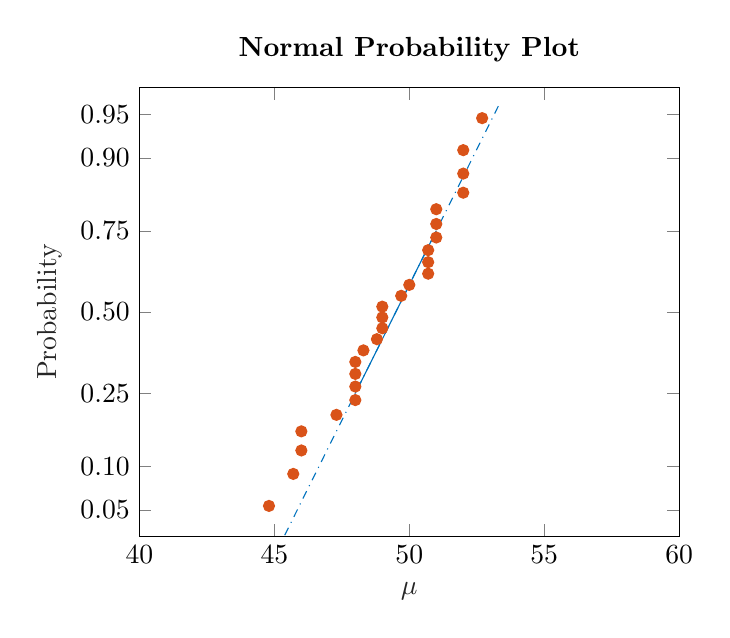
\begin{tikzpicture}

\begin{axis}[%
\plotsettings
xmin=40,
xmax=60,
xlabel style={font=\color{white!15!black}},
xlabel={$\mu$ \si{\decibel}},
ymin=-1.86273186742165,
ymax=1.86273186742165,
ytick={-3.09023230616781,-2.74778138544499,-2.32634787404084,-2.05374891063182,-1.64485362695147,-1.2815515655446,-0.674489750196082,0,0.674489750196082,1.2815515655446,1.64485362695147,2.05374891063182,2.32634787404084,2.74778138544499,3.09023230616781},
yticklabels={{0.001},{0.003},{0.01},{0.02},{0.05},{0.10},{0.25},{0.50},{0.75},{0.90},{0.95},{0.98},{0.99},{0.997},{0.999}},
ylabel style={font=\color{white!15!black}},
ylabel={Probability},
title style={font=\bfseries},
title={Normal Probability Plot},
legend style={legend cell align=left, align=left, draw=white!15!black} %at={(0.045,0.669)}, anchor=south west, 
legend entries={Gaussian Fit, Subject Data}
legend pos=south east
]

\addlegendimage{mycolor1},
\addlegendimage{only marks,mycolor2},

\addplot [color=mycolor1]
  table[row sep=crcr]{%
48	-0.675557426684197\\
51	0.675557426684197\\
};
%\addlegendentry{Normal Distribution}

\addplot [color=mycolor2, draw=none, mark=*, mark options={solid, mycolor2}]
  table[row sep=crcr]{%
42	-2.10016549284447\\
44.8	-1.61116916235268\\
45.7	-1.34516663417664\\
46	-1.15034938037601\\
46	-0.991526474677331\\
47.3	-0.85444739869599\\
48	-0.731808083859618\\
48	-0.619306769508776\\
48	-0.514156100744534\\
48	-0.414413329600076\\
48.3	-0.318639363964375\\
48.8	-0.225707953860159\\
49	-0.13468979400892\\
49	-0.0447761766955162\\
49	0.0447761766955164\\
49.7	0.13468979400892\\
50	0.225707953860159\\
50.7	0.318639363964375\\
50.7	0.414413329600076\\
50.7	0.514156100744534\\
51	0.619306769508776\\
51	0.731808083859618\\
51	0.85444739869599\\
52	0.991526474677331\\
52	1.15034938037601\\
52	1.34516663417664\\
52.7	1.61116916235268\\
53.3	2.10016549284447\\
};
%\addlegendentry{Subject}



\addplot [color=mycolor1, dashdotted]
  table[row sep=crcr]{%
42	-3.37778713342098\\
53.3	1.71141214759996\\
};
%\addlegendentry{data1}





\end{axis}
\end{tikzpicture}%
		\caption{The plot shows the Gaussian  \gls{pdf} as the blue line with the initial data in \autoref{sec:pdf_of_bc}. The histogram is based on the mean data merge of \autoref{apend:matching_in_bier} and \autoref{apend:match_field_init}}
		\label{fig:total_normplot}
\end{figure}

It can be seen in \autoref{fig:total_pdf} and \autoref{fig:total_normplot} that the measured data for the total data have the same tendency as all data separated. The calculated \gls{mse} between the data and the Gaussian distribution function in this case is $7.7464 \cdot 10^{-5}$ and it can also be seen that the subject data compare to the \gls{cdf} mostly follows the line. Compare to the data present in the three non merged data, the \gls{mse} converging to a higher Gaussian distribution fit so lower \gls{mse}. There is no outliers and the highest probability lays close to the highest probability of the Gaussian distribution. 

To present the 25 \textsuperscript{th} and 75 \textsuperscript{th} percentile, the median of the total data and the \SI{99.3}{\percent} coverage a boxplot is calculated and visualized in \autoref{fig:total_box}.

 \begin{figure}[H]
	\centering
	% This file was created by matlab2tikz.
%
%The latest updates can be retrieved from
%  http://www.mathworks.com/matlabcentral/fileexchange/22022-matlab2tikz-matlab2tikz
%where you can also make suggestions and rate matlab2tikz.
%
\begin{tikzpicture}

\begin{axis}[%
width=120mm, 
height=50mm, 
at={(5mm,5mm)}, 
scale only axis,
xmin=41.435,
xmax=53.865,
xlabel style={font=\color{white!15!black}},
xlabel={$\mu$ \si{\decibel}},
ylabel style={font=\color{white!15!black}},
ylabel={Total data},
ymin=0.5,
ymax=1.5,
ytick={1},
axis background/.style={fill=white},
legend style={legend cell align=left, align=left, draw=white!15!black}
]
\addplot [color=black, dashed, forget plot]
  table[row sep=crcr]{%
51	1\\
53.3	1\\
};
\addplot [color=black, dashed, forget plot]
  table[row sep=crcr]{%
44.8	1\\
48	1\\
};
\addplot [color=black, forget plot]
  table[row sep=crcr]{%
53.3	0.9625\\
53.3	1.0375\\
};
\addplot [color=black, forget plot]
  table[row sep=crcr]{%
44.8	0.9625\\
44.8	1.0375\\
};
\addplot [color=blue, forget plot]
  table[row sep=crcr]{%
48	0.925\\
51	0.925\\
51	1.075\\
48	1.075\\
48	0.925\\
};
\addplot [color=red, forget plot]
  table[row sep=crcr]{%
49	0.925\\
49	1.075\\
};
\addplot [color=black, draw=none, mark=+, mark options={solid, red}, forget plot]
  table[row sep=crcr]{%
42	1\\
};
\end{axis}
\end{tikzpicture}%
		\caption{The plot shows a box and whisker plot of the data merge of \autoref{apend:matching_in_bier} and \autoref{apend:match_field_init}}
		\label{fig:total_box}
\end{figure}


In \autoref{fig:total_box} it can be seen that there is only one outliers from the \SI{99.3}{\percent} coverage, the 25 \textsuperscript{th} percentile lies at \SI{48}{\decibel} and the 75 \textsuperscript{th} percentile lies at \SI{51}{\decibel}. From the data in the initial test and the familiarization the subject data do have a uniformly distribution within the subject mean range, but by analyse the total data and the boxplot, the Gaussian hypnotises can be assumed.


\section{Conclusion}
It can be concluded that the matching part for the \gls{bier} test might converge to a normal distribution by observing the \gls{mse} and locking at the boxplot. It can also be concluded that with the measured subject the mean level for the \gls{bc} is \SI{49.1}{\decibel} to match the air and the variance level is \SI{6.82}{\decibel}. The standard deviation of the subject data is \SI{2.61}{\decibel} and the \SI{50}{\percent} of the subject result lies within \SI{48}{\decibel} to \SI{51}{\decibel}.





